\chapter*{Proposition 19}
\label{prop:19}

\begin{figure*}[ht]
    \begin{center}
    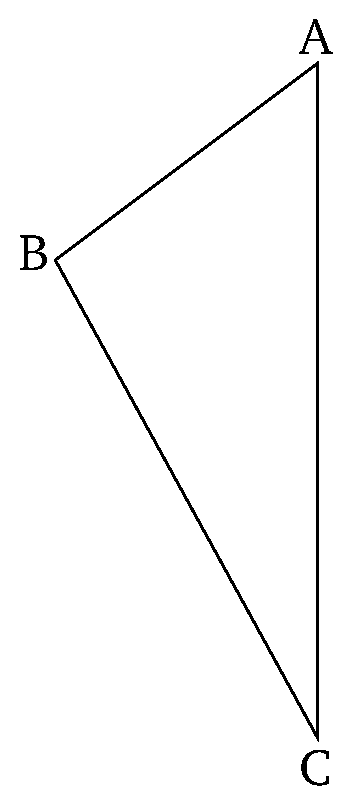
\includegraphics[width=0.5\linewidth]{figures/fig19e.eps}
    \label{fig:prop_19}
    \end{center}
\end{figure*}

In any triangle, the greater angle is subtended by the greater side.

Let $ABC$ be a triangle having the angle $ABC$ greater than $BCA$. I say
that side $AC$ is also greater than side $AB$.

For if not, $AC$ is certainly either equal to, or less than, $AB$. In fact, $AC$ is not
equal to $AB$. For then angle $ABC$  would also have been equal to $ACB$ [Prop.~1.5].
But it is not. Thus, $AC$ is not equal to $AB$.
Neither, indeed, is $AC$ less than $AB$. For then angle $ABC$ would also have been
less than $ACB$ [Prop.~1.18]. But it is not. Thus, $AC$ is not less than
$AB$. But it was  shown that ($AC$) is    not equal (to $AB$) either. Thus, $AC$ 
is greater than $AB$.

Thus, in any triangle, the greater angle is subtended by the greater side.
(Which is) the very thing it was required to show.


\section*{Commentary}

\begin{proposition}\label{proposition_19}\lean{Elements.Book1.proposition_19}\leanok
    In $\triangle~ABC$, if $\angle~ABC~>~\angle~BCA$, then |AC|~>~|AB|.
\end{proposition}
\begin{proof}
    \uses{proposition_5',proposition_18}\leanok
    See the original proof by Euclid.
\end{proof}
